\chapter{Forskningsmetoder og forskningsdesign}
\label{ch:method}

I dette kapittelet presenteres og drøftes forskningsmetodene og forskningsdesignet til studien.
I tillegg diskuteres validiteten til forskningen. 
Som skrevet tidligere, bygger forskningsprosessen på boken «Researching Information Systems and Computing» \citep{oates} (se figur \ref{fig:oates_model}).

\iffalse
I en forskningsartikkel er avsnittet om metode ofte det viktigste. Det samme gjelder metodekapitlet i en empirisk oppgave. Dette kan også være et vanskelig kapittel å skrive, fordi det ikke alltid er klart hvilken «jobb» det skal gjøre. Et metodekapittel skal ikke gjengi innholdet i fagets metodebøker. Dersom du har brukt intervju er det for eksempel ikke nødvendig å liste opp forskjellige typer forskningsintervju. Du trenger heller ikke redegjøre for forskjellene mellom kvantitative og kvalitative metoder, eller liste opp ulike typer validitet og reliabilitet.

Det du skal gjøre, er å vise hvordan dine valg av design og metode egner seg til å belyse/besvare ditt forskningsspørsmål, og hvilke vurderinger du har foretatt mht validitet (gyldighet) og reliabilitet (pålitelighet).’Show, don’t tell’ – vis leseren hva du gjorde, og forklar hvorfor. Da vil metodekapitlet sette de ulike delene av oppgaven i sammenheng, og det blir spennende å lese. I praksis betyr dette å demonstrere at du har forstått den praktiske betydningen av begrepene.

Et godt metodekapittel forteller hva du har gjort i din undersøkelse, og forklarer hvorfor. Hvordan samlet du inn data? Hva kan man forvente å finne ved å gjøre det på denne måten?
Hva var rammene? Hvilke avveininger måtte tas? Hva oppnår du ved å bruke denne metoden?
Vis hva du har gjort for å øke validiteten. Hva kan du si om reliabiliteten (påliteligheten) i datainnsamlingen? Hvordan vet du at du har undersøkt det du ønsket å undersøke? Hvilke slutninger kan trekkes på dette grunnlaget? Hvilke slutninger er sikre, og hvilke er mer tentative? Hvilken overføringsverdi har resultatene? Kan du generalisere – hvorfor, hvorfor ikke?
Svakheter og styrker ved metoden skal beskrives. Den ekstra gode oppgaven utmerker seg ved å forsvare sine valg og samtidig kritisere dem.

Formål
Produkter (bidrag/resultater)
Prosess
Deltakere
Paradigme
Presentasjon
\fi

%[width=0.85\textwidth,center]
\begin{figure}
\centering
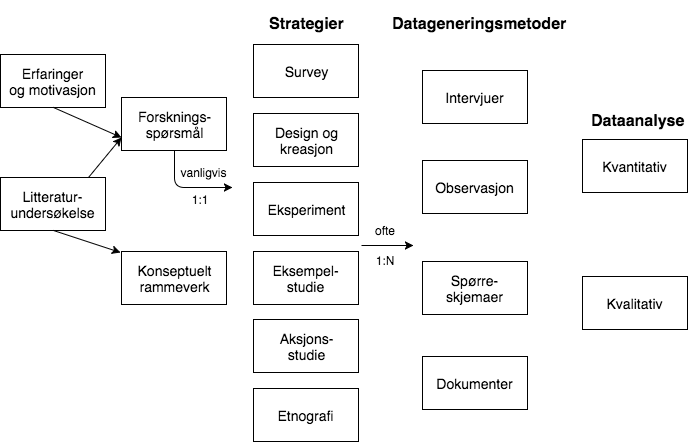
\includegraphics[width=\textwidth]{fig/oates/oates_research_norwegian}
\caption{Modell av forskningsprosessen fra \citet{oates}.}
\label{fig:oates_model}
\end{figure}

\section{Forskningsstrategier}
Som skrevet i kapittel \ref{ch:introduction}, er formålet med denne forskningen å undersøke hvordan ny teknologi basert
på \gls{iot}-skyløsninger kan brukes til avstandsoppfølging med prosjektet til Trondheim kommune som ramme. Dermed er å lage noe nytt,
«design og kreasjon», en naturlig hovedstrategi. Den støttende understrategien er en eksempelstudie av Trondheims kommunes arbeid
med avstandsoppfølging. De to strategiene er kort under.

\subsection{Design og kreasjon av et pulsoksimeter}
Ulempen med å velge denne strategien er at det er fort gjort at en kun demonstrerer
teknisk kompetanse uten at det kvalifiserer som god forskning. I tillegg til det nye produktet må ny kunnskap utvikles, bygget på analyse, argumenter
og kritiske evalueringer \citep[s. 109]{oates}.
\blindtext

\subsection{Trondheim kommune -- en eksempelstudie}
\blindtext

\section{Forskningsspørsmål}
\subsection{Forskningsspørmål 1}
\subsection{Forskningsspørmål 2}
\subsection{Forskningsspørmål 3}
\subsection{Forskningsspørmål 4}

\section{Forskningsdesign}
\blindtext

\section{Brukersentrert utvikling}
\blindtext

\section{Case-studie}
\blindtext

\section{Intervjuer}
\blindtext

\section{Fokusgrupper}
\blindtext
